\section{Experiment und Durchf\"uhrung}
Hier steht die Dokumentation des experimentellen Aubaus und evtl. wichtige 
Bemerkungen zur Durchf\"uhrung der Messung.

Statt dessen stehen hier Beispiele zu Grafiken.

Wichtig ist, das Bilder (oder auch Tabellen) in Latex nicht an einer festen Stelle stehen sollten, sondern sich bewegen \glqq floaten\grqq\ können, um
% \glqq \grqq macht "deutsche" Anführungszeichen  
ein besseres Layout zu erreichen. Man bezeichnet Figuren und Bilder deshalb auch als Floats.

% Wir definieren eine Bildumgebung
% [ tbhp ] sagt, das das Bild bevorzugt oben (t), unten (b), hier (h)
% oder auf einer neuen Seite angeordnet werden soll. Die Reihenfolge 
% ist maßgeblich
\begin{figure}[tbp]
% damit zentrieren wir das Bild
 \centering
% jetzt fügen wir ein Bild ein
 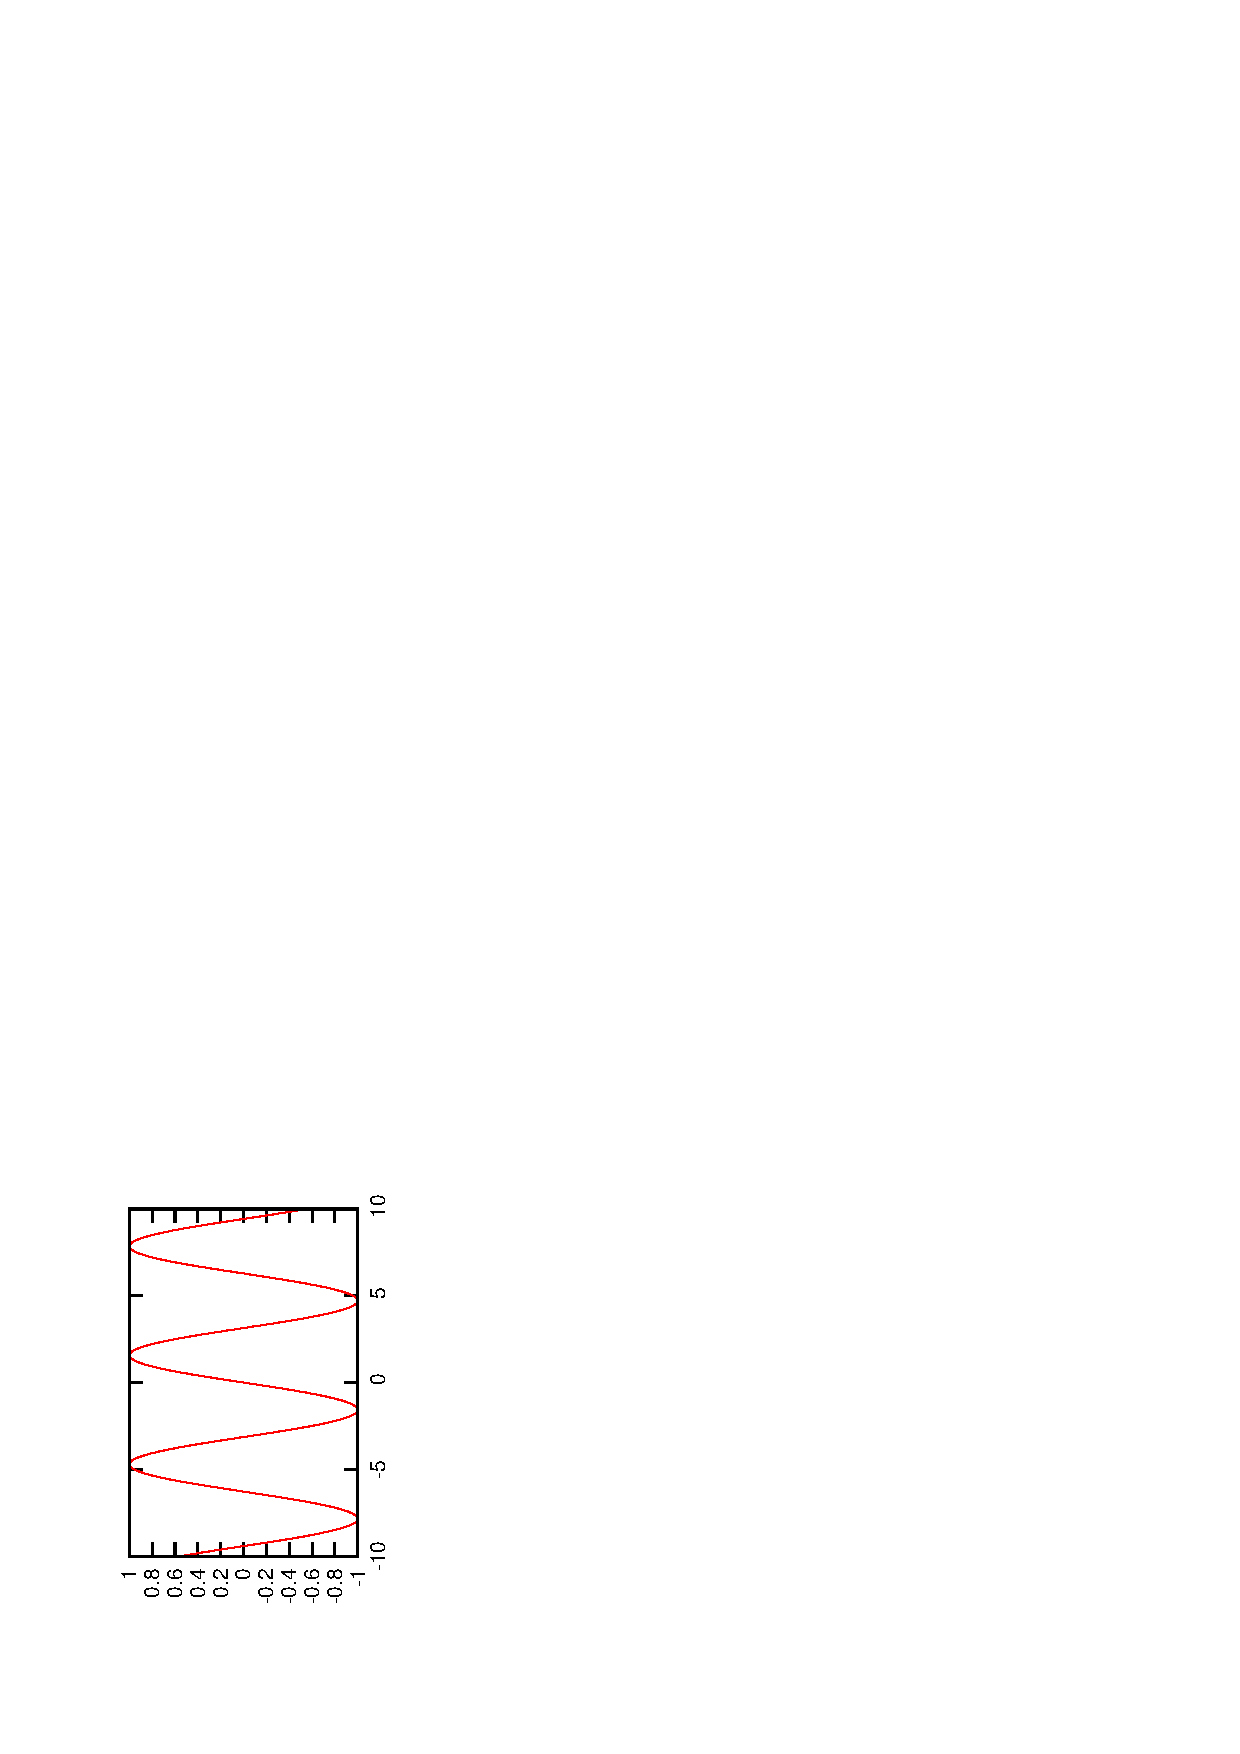
\includegraphics[angle=270, width=5cm]{sinus} 
% Die Dateiendung fehlt, es wird automatisch das eps oder pdf gewählt
 \caption[Kurz: Eine Sinuskurve]
 {Lang: Dieses Bild zeigt eine Sinuskurve mit 
drei periodischen Schwingungen. Es ist 5\,cm breit. Das Bild musste um 
270\textdegree  gedreht werden. Es müsste breiter sein!}
% in eckigen Klammern steht eine Kurzbezeichnung, wie sie in einem 
% Abbildungsverzeichnis stehen köšnnte
% Wichtig ist, dass \caption eine Nummer füŸr das Bild erstellt, 
% erst dann kann man ein label darauf setzen!
\label{fig:sinus}
\end{figure}

\begin{figure}[bh]
 \centering
 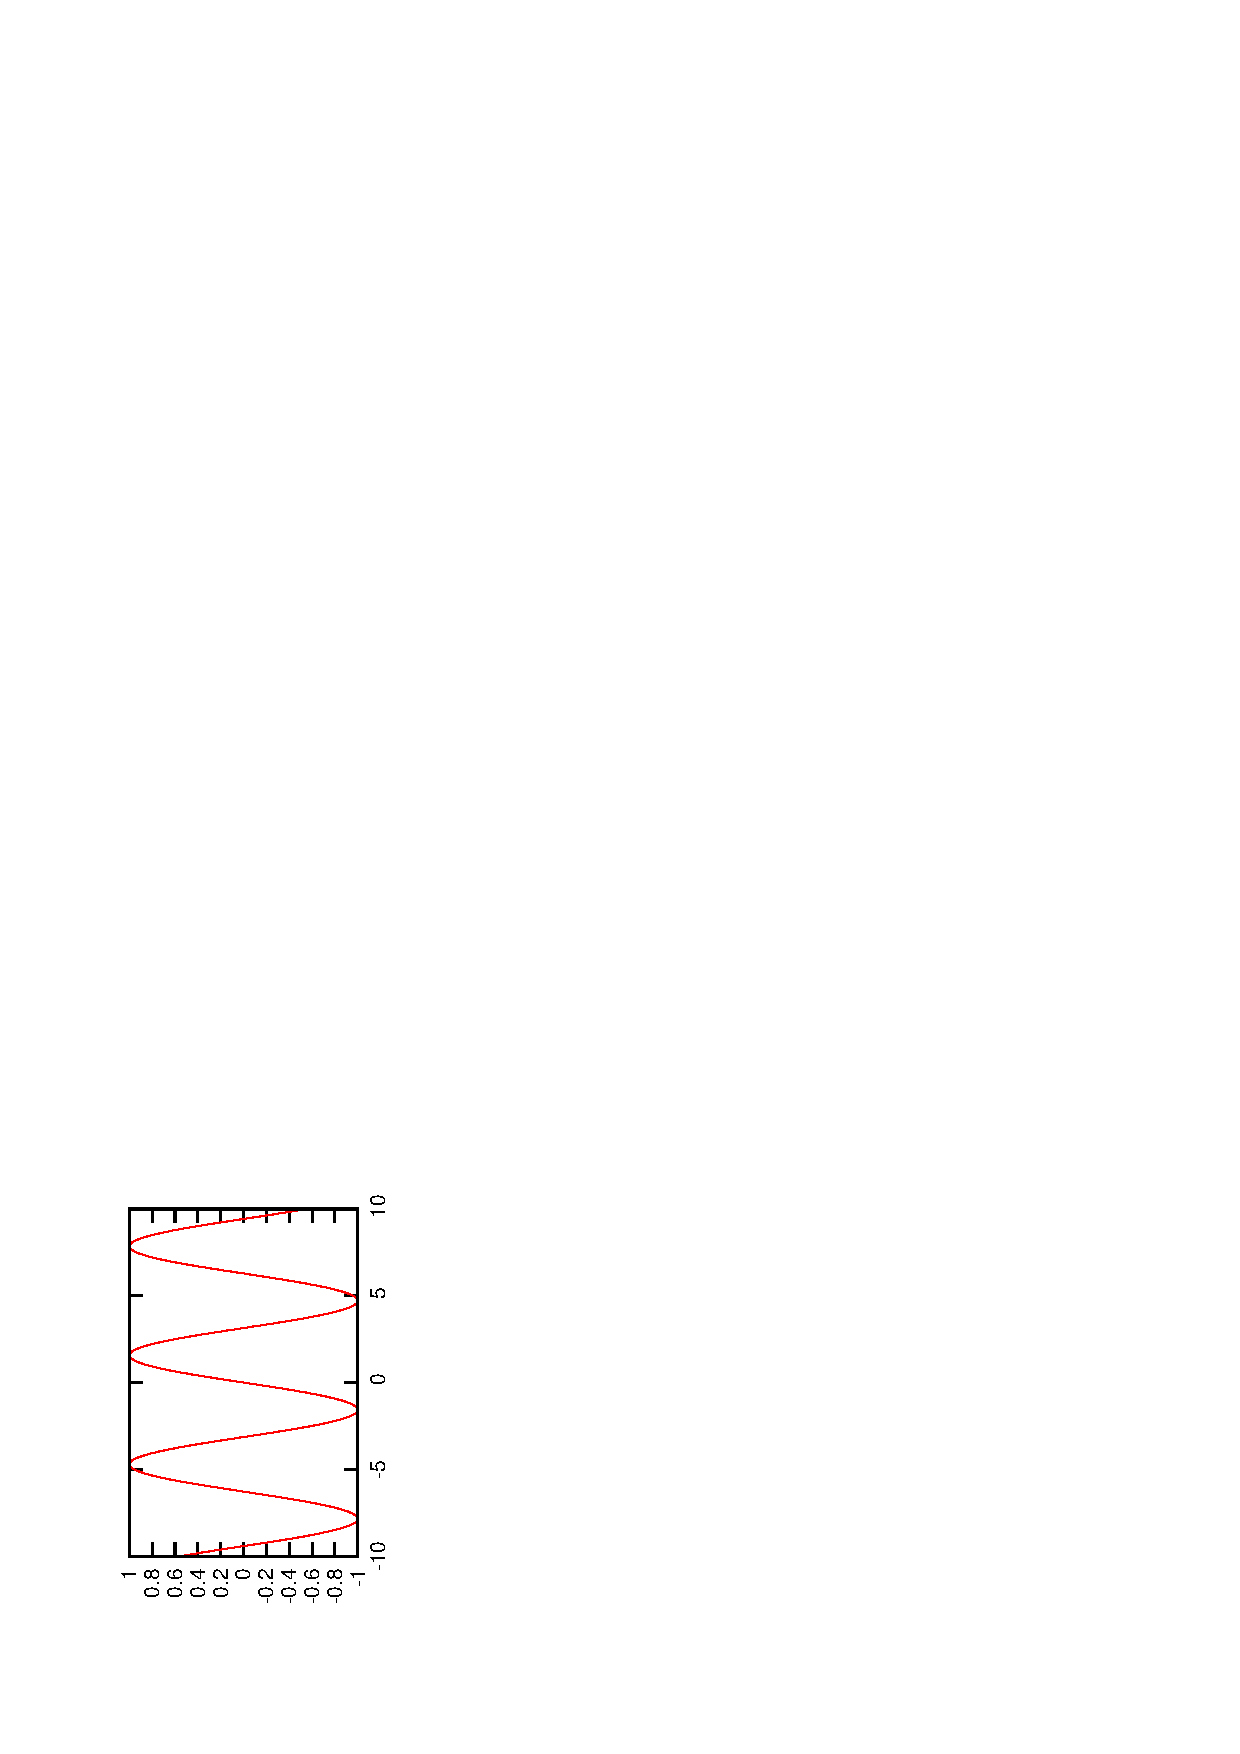
\includegraphics[angle=255, width=0.25\linewidth]{sinus}
  \caption{Dieses Bild misst 25\%  der Textbreite und ist um 200\textdegree gedreht.}
 \label{fig:sinus2}
\end{figure}
Bilder haben \textbf{grundsätzlich} Unterschriften!
Schlecht ist, dass dieses Bild keine Achsenbeschriftung hat!